\documentclass[11pt]{article}

\usepackage{graphicx}
\usepackage{amsmath}
\usepackage[margin=0.8in]{geometry}
\usepackage{float}


\usepackage{listings}
\usepackage{xcolor}

\definecolor{codegreen}{rgb}{0,0.6,0}
\definecolor{codegray}{rgb}{0.5,0.5,0.5}
\definecolor{codepurple}{rgb}{0.58,0,0.82}
\definecolor{backcolour}{rgb}{0.95,0.95,0.92}

\lstdefinestyle{mystyle}{
	backgroundcolor=\color{backcolour},   
	commentstyle=\color{codegreen},
	keywordstyle=\color{magenta},
	numberstyle=\tiny\color{codegray},
	stringstyle=\color{codepurple},
	basicstyle=\ttfamily\footnotesize,
	breakatwhitespace=false,         
	breaklines=true,                 
	captionpos=b,                    
	keepspaces=true,                 
	numbers=left,                    
	numbersep=5pt,                  
	showspaces=false,                
	showstringspaces=false,
	showtabs=false,                  
	tabsize=2
}

\usepackage{tikz}
\usetikzlibrary{shapes.geometric, arrows}
\tikzstyle{startstop} = [rectangle, rounded corners, minimum width=3cm, minimum height=1cm,text centered, draw=black, fill=red!30]
\tikzstyle{ISR} = [rectangle, rounded corners, minimum width=3cm, minimum height=1cm,text centered, draw=black, fill=green!30]
\tikzstyle{io} = [trapezium, trapezium left angle=70, trapezium right angle=110, minimum width=1cm, minimum height=1cm, text centered, draw=black, fill=blue!30]
\tikzstyle{process} = [rectangle, minimum width=3cm, minimum height=1cm, text centered, draw=black, fill=orange!30]
\tikzstyle{arrow} = [thick,->,>=stealth]


\lstset{style=mystyle}

\title{MECH 423 Final Project \\
		The No Excuses Waking Up System}
\author{Dana Deutsch - 10631166\\
		deutschdana@gmail.com}
\date{November 1st 2020}
\begin{document}
\maketitle
\newpage
\tableofcontents
\newpage

\section{Objectives}
The goal of this project is to create an alarm clock system for people who have a hard time waking up and getting out of bed.
Many people simply turn off their alarms and fall back asleep.
Then they must to set multiple alarms at various intervals to remind themselves to get up.
This is a temporary solution since you can still turn off all the alarm and stay in bed.
My objective of my system is to eliminate the possibility of remaining in bed by taking away the power to fully "turn off" the alarm while keeping a short "snooze" functionality. 
The reason for the snooze is because people enjoy laying in bed for a few minutes before fully waking up and a consistent alarm while in bed will get annoying. 
Since most people don't use a physical alarm clock and instead use their phones, this system will work best if it were to interface with the phone people already use.\\

Creating a phone application interface is outside the scope of this project as it adds a lot much functions and complexity for the short timeline provided. 
Instead the goal of the project is to use the phone alarm sound as a trigger point for an bed detecting alarm system which operates separate from the phone,
This way the main alarm can be set on the phone which users already have set up since it has a better interface and more alarm features.
However , the device run on the a microcontroller still operates in respect to the phone. 
The device will sense when the phone alarm goes off in order to begin its functions instead of having its own internal real time clock and alarm setting capacity.  
After the original alarm, the device will periodically ring after the user "snoozes" until the user leaves the bed and doesn't return to bed for a set amount of time. 
The device will look like a small box that is placed by the bed right where the user normally places their phone to charge.
The device will have small wires leading to sensors under the bed to connect to the detection circuitry.

\section{Rationale}
I want to make this device since it solves a problem I face daily along with many other people.
Instead of setting up 5 different alarms which are close together and spread out to make sure I get up, I can use this device.
I sometimes ignore my alarms and just decide to keep sleeping so this way I will be forced to get up and hopefully fix my sleeping scheduled.
This product isn't available on the market right so its only achievable by making it myself.
I hope this project will provide a concept functionality prototype for a possible market device that uses this method or a better phone app interface. 
As well many home automation can be made using the bed occupancy detection function like starting the coffee maker when you leave the bed.
An example of how I imagine a final product to look like is found in Figure \ref{fig:market}.

\begin{figure}[H]
	\centering
	%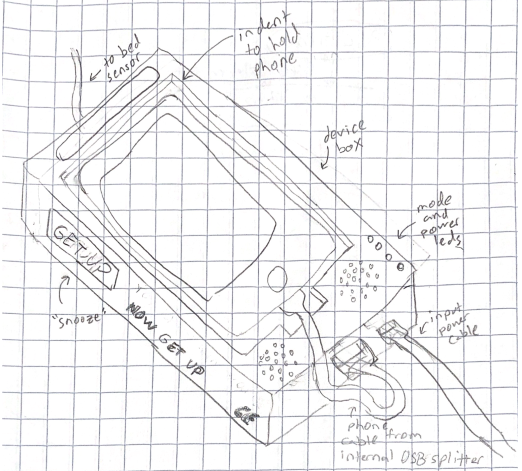
\includegraphics[width = 0.5\linewidth]{marketSolution}
	\caption{Concept Drawing For a Alternative Version of the Device Integrated in a Phone Charging Station}
	\label{fig:market}
\end{figure}

\begin{figure}[H]
	\centering
	\label{fig:flow}
	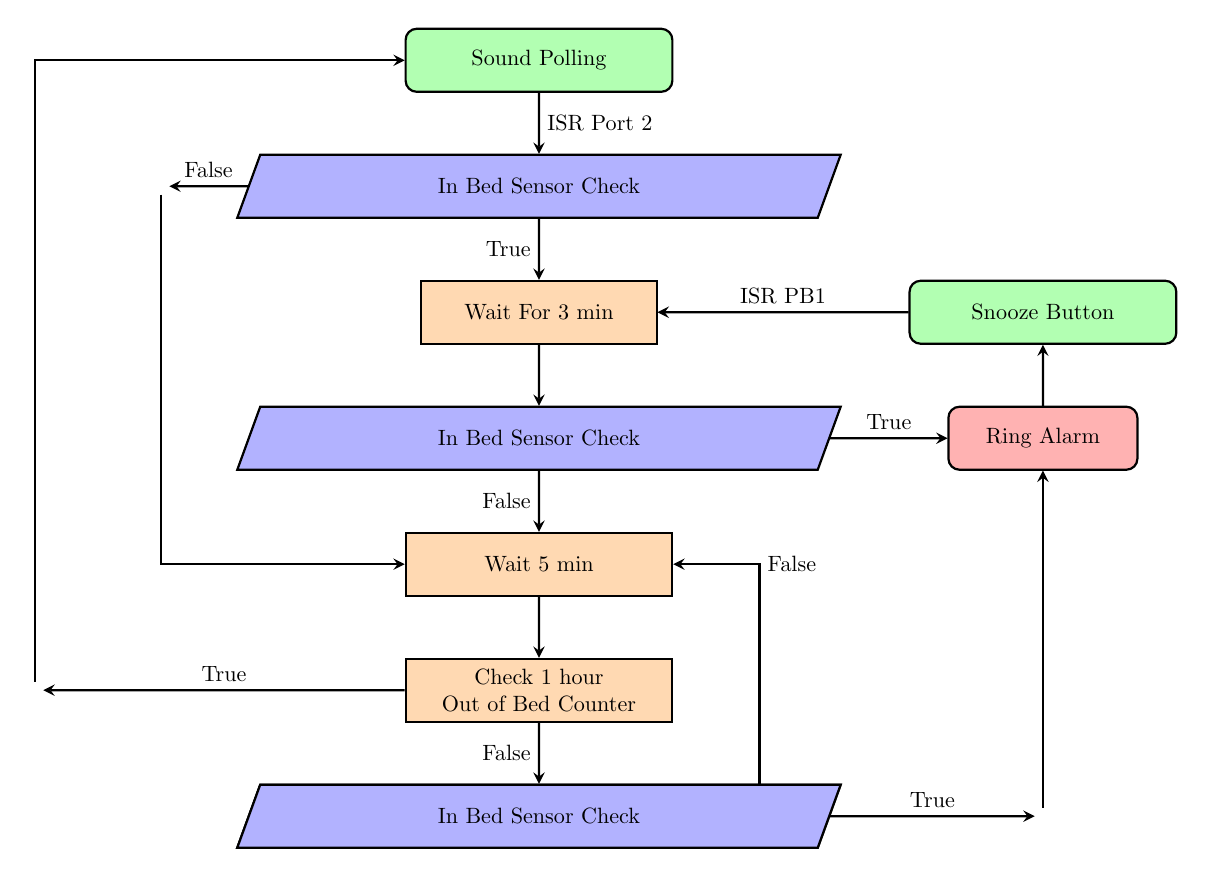
\begin{tikzpicture}[node distance =2cm, thick,scale=0.9, every node/.style={scale=0.8}]
		
		\node (Realtime) [ISR,text width=4cm ] {Sound Polling}; 
		\node (InBed3) [io, below of=Realtime,text width=4cm] {In Bed Sensor Check};	
		\node (Wait1) [process, below of=InBed3,text width=3.5cm] {Wait For 3 min };
		\node (snoozePB) [ISR, right of=Wait1,text width=4cm, xshift = 6cm] {Snooze Button};
		\node (InBed) [io, below of=Wait1,text width=4cm] {In Bed Sensor Check}; 
		\node (Ring1) [startstop, right of =InBed, xshift = 6cm] {Ring Alarm};
		\node (wait2) [process, below of=InBed, text width=4cm] {Wait 5 min};
		\node (counter) [process, below of=wait2, text width=4cm] {Check 1 hour \\Out of Bed Counter};
		\node (InBed2) [io, below of=counter, text width=4cm] {In Bed Sensor Check}; 
		\node (return1) [right of=InBed2, xshift =6cm]{};
		\node (return2) [left of=counter, xshift =-6cm]{};
		\node (return3) [left of=InBed3, xshift =-4cm]{};
		\node (return4) [right of=InBed2, xshift = 1.5cm]{};
		
		
		\draw [arrow] (Realtime) -- node[anchor=west] {ISR Port 2}(InBed3);
		\draw [arrow] (InBed3) -- node[anchor=east] {True}(Wait1);
		\draw [arrow] (InBed3) -- node[anchor=south] {False}(return3);
		\draw [arrow] (return3) |- (wait2);
		\draw [arrow] (Wait1) -- (InBed);
		\draw [arrow] (Ring1) -- (snoozePB);
		\draw [arrow] (snoozePB) -- node[anchor=south]{ISR PB1} (Wait1);
		\draw [arrow] (InBed) -- node[anchor=south] {True} (Ring1);
		\draw [arrow] (InBed) -- node[anchor=east] {False} (wait2);
		\draw [arrow] (wait2) --  (counter);
		\draw [arrow] (counter) -- node[anchor=south] {True} (return2);
		\draw [arrow] (counter) -- node[anchor=east] {False}(InBed2);
		\draw [arrow] (return1) -- (Ring1);	
		\draw [arrow] (InBed2) -- node[anchor=south]{True}(return1);	
		\draw [arrow] (return2) |- (Realtime);
		\draw [arrow] (return4) |- node[anchor=west]{False} (wait2);
		\node (InBed5) [io, below of=counter, text width=4cm] {In Bed Sensor Check}; 
	\end{tikzpicture}
	\caption{Flowchart for the Alarm Actuation Logic}
\end{figure}


It takes 4 sec for average lets remove that, 

\end{document}